%=====================================================================
%  01-SAMPUL.TEX — SLIDE JUDUL
%=====================================================================
%  Isi slide judul diambil OTOMATIS dari konfigurasi.tex melalui
%  perintah \titlepage (judul, penulis, institusi, tanggal, logo).
%  Yang diatur di sini hanya latar belakang dan penempatan logo.
%=====================================================================

\section{}   % Bagian kosong: slide sampul tidak muncul di navigasi

%--- 1) LATAR BELAKANG -----------------------------------------------
%  \transparent{0.2} = 20% pekat (makin kecil makin pudar), agar teks
%  judul tetap terbaca di atas foto kampus.
\usebackgroundtemplate{%
    \transparent{0.2}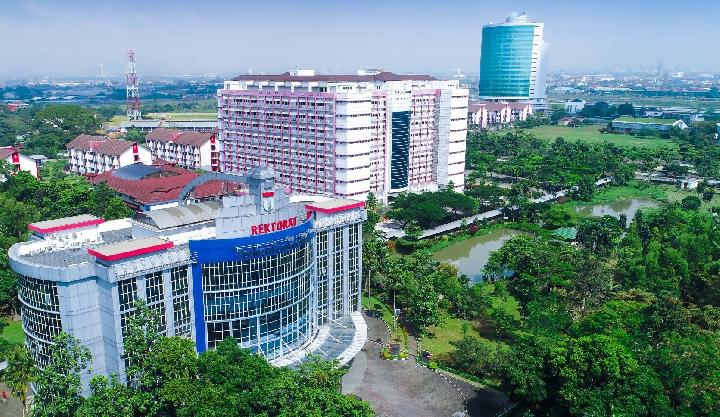
\includegraphics[width=\paperwidth]{gambar/logo/telkom.jpg}%
}

%--- 2) SEMBUNYIKAN LOGO POJOK (khas slide sampul) -------------------
\logo{}

%--- 3) SLIDE JUDUL --------------------------------------------------
\begin{frame}
    \vspace{-0.25cm}
    \titlepage   % <-- otomatis dari konfigurasi.tex

    % Tiga logo institusi di bagian atas slide.
    % \node[inner sep=0pt] at (x,y){gambar}; -- koordinat dalam cm,
    % kertas 16:9 berukuran 16cm x 9cm, titik (0,0) di TENGAH slide.
    % (gambar tidak memakan ruang: overlay = mengambang di atas slide)
    \begin{tikzpicture}[overlay,remember picture]
        \node[inner sep=0pt] at (4.0,7.6){%
            
\includegraphics[width=2.0cm]{gambar/logo/TELU Horizontal.png}};
        \node[inner sep=0pt] at (8.0,7.6){%
            
\includegraphics[width=2.8cm]{gambar/logo/Logo_AICOMS_Telkom_University.png}};
        \node[inner sep=0pt] at (12.0,7.6){%
            
\includegraphics[width=2.0cm]{gambar/logo/TELU Horizontal.png}};
    \end{tikzpicture}
\end{frame}

%--- 4) KEMBALIKAN TAMPILAN UNTUK SLIDE ISI --------------------------
\usebackgroundtemplate{}   % hapus latar belakang foto

% Logo kepoloan muncul kembali di pojok kanan-atas setiap slide isi
\addtobeamertemplate{headline}{}{%
    \begin{tikzpicture}[remember picture,overlay]
        \node[anchor=north east] at (current page.north east) {%
            
\includegraphics[width=0.5cm]{gambar/logo/TELU Vertikal.png}%
        };
    \end{tikzpicture}%
}

% Warna headline untuk slide isi (emas di atas putih)
\setbeamercolor{section in head/foot}{fg=scisGold, bg=white}
\setbeamercolor{title in head/foot}{fg=white, bg=scisGold}
\setbeamercolor{headline}{fg=scisGold, bg=white}
